\documentclass[border=0pt]{standalone}
\usepackage{lmodern}
\usepackage{tikz}
\usepackage{pgfplots}
\usepgfplotslibrary{groupplots}
\pgfplotsset{compat=1.17}
\definecolor{f07min}{HTML}{000000}
\definecolor{f07sg}{HTML}{0072B2}
\definecolor{f07arpls}{HTML}{D55E00}
\begin{document}
\begin{minipage}{181.86mm}
\centering
% figure: P08-F07; panel: f07-pooled-four-fold-m01-p05-selected; semantic-sha256: a80ccd58447783b6ff83336d15c300b5297f955760921573638eaca3cc08512e
{\bfseries\fontsize{10}{12}\selectfont P08-F07 / RQ-S05 | Source-selected CNN | M01 individual-spectrum predictions | Pooled sensitivity (S)\par}
\vspace{2mm}
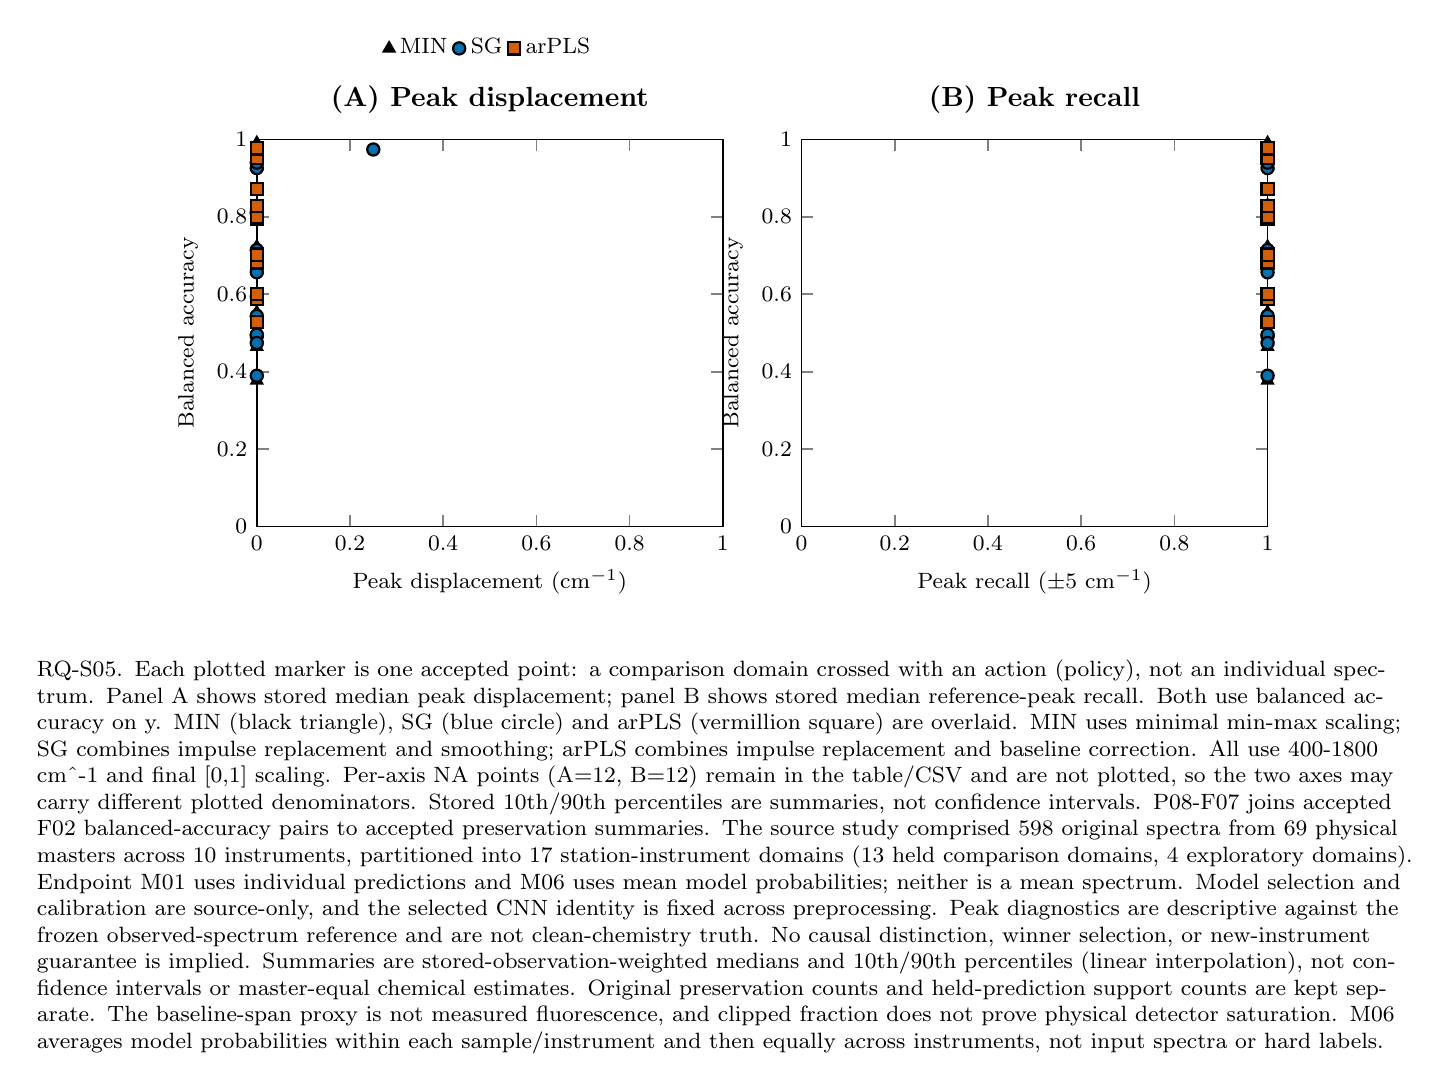
\begin{tikzpicture}
\begin{groupplot}[group style={group size=2 by 1, horizontal sep=10mm, vertical sep=0mm}, width=75mm, height=65mm, clip=false, axis line style={line width=0.6pt}, tick style={line width=0.6pt}, tick label style={font=\fontsize{8}{9.6}\selectfont, black}, label style={font=\fontsize{8}{9.6}\selectfont, black}, title style={font=\bfseries\fontsize{10}{12}\selectfont}, legend style={at={(0.5,1.18)}, anchor=south, draw=none, fill=none, legend columns=3, font=\fontsize{8}{9.6}\selectfont}, ymin=0, ymax=1, ytick={0,0.20000000000000001,0.40000000000000002,0.59999999999999998,0.80000000000000004,1}, yticklabels={0,0.2,0.4,0.6,0.8,1}]
\nextgroupplot[title={(A) Peak displacement}, xlabel={Peak displacement (cm$^{-1}$)}, ylabel={Balanced accuracy}, xmin=0, xmax=1, xtick={0,0.20000000000000001,0.40000000000000002,0.59999999999999998,0.80000000000000004,1}, xticklabels={0,0.2,0.4,0.6,0.8,1}]
\addlegendimage{only marks, mark=triangle*, mark size=2.2pt, mark options={fill=f07min, draw=black, line width=0.8pt}}
\addlegendentry{MIN}
\addlegendimage{only marks, mark=*, mark size=2.2pt, mark options={fill=f07sg, draw=black, line width=0.8pt}}
\addlegendentry{SG}
\addlegendimage{only marks, mark=square*, mark size=2.2pt, mark options={fill=f07arpls, draw=black, line width=0.8pt}}
\addlegendentry{arPLS}
\addplot+[only marks, mark=triangle*, mark size=2.2pt, mark options={fill=f07min, draw=black, line width=0.8pt}] coordinates {(0,0.49682539682539684) (0,0.48723809523809525) (0,0.55103030303030298) (0,0.8053030303030303) (0,0.9310023310023311) (0,0.37741397849462366) (0,0.8294973544973544) (0,0.99047619047619051) (0,0.46455026455026455) (0,0.55286195286195283) (0,0.94999999999999996) (0,0.72253968253968248) (0,0.67528735632183912)};
\addplot+[only marks, mark=*, mark size=2.2pt, mark options={fill=f07sg, draw=black, line width=0.8pt}] coordinates {(0,0.49301587301587302) (0,0.49572486772486773) (0,0.54424242424242419) (0,0.81136363636363629) (0,0.92587412587412599) (0,0.3897150537634409) (0,0.80945767195767204) (0.25,0.97380952380952368) (0,0.47407407407407404) (0,0.59461279461279459) (0,0.94000000000000006) (0,0.71420634920634918) (0,0.65680076628352491)};
\addplot+[only marks, mark=square*, mark size=2.2pt, mark options={fill=f07arpls, draw=black, line width=0.8pt}] coordinates {(0,0.59738095238095235) (0,0.58831746031746035) (0,0.60145454545454546) (0,0.7936363636363637) (0,0.8717948717948717) (0,0.68582258064516144) (0,0.80039682539682533) (0,0.95238095238095233) (0,0.52910052910052907) (0,0.68215488215488229) (0,0.97666666666666679) (0,0.70230158730158732) (0,0.82796934865900373)};
\nextgroupplot[title={(B) Peak recall}, xlabel={Peak recall ($\pm$5 cm$^{-1}$)}, ylabel={Balanced accuracy}, xmin=0, xmax=1, xtick={0,0.20000000000000001,0.40000000000000002,0.59999999999999998,0.80000000000000004,1}, xticklabels={0,0.2,0.4,0.6,0.8,1}]
\addplot+[only marks, mark=triangle*, mark size=2.2pt, mark options={fill=f07min, draw=black, line width=0.8pt}] coordinates {(1,0.49682539682539684) (1,0.48723809523809525) (1,0.55103030303030298) (1,0.8053030303030303) (1,0.9310023310023311) (1,0.37741397849462366) (1,0.8294973544973544) (1,0.99047619047619051) (1,0.46455026455026455) (1,0.55286195286195283) (1,0.94999999999999996) (1,0.72253968253968248) (1,0.67528735632183912)};
\addplot+[only marks, mark=*, mark size=2.2pt, mark options={fill=f07sg, draw=black, line width=0.8pt}] coordinates {(1,0.49301587301587302) (1,0.49572486772486773) (1,0.54424242424242419) (1,0.81136363636363629) (1,0.92587412587412599) (1,0.3897150537634409) (1,0.80945767195767204) (1,0.97380952380952368) (1,0.47407407407407404) (1,0.59461279461279459) (1,0.94000000000000006) (1,0.71420634920634918) (1,0.65680076628352491)};
\addplot+[only marks, mark=square*, mark size=2.2pt, mark options={fill=f07arpls, draw=black, line width=0.8pt}] coordinates {(1,0.59738095238095235) (1,0.58831746031746035) (1,0.60145454545454546) (1,0.7936363636363637) (1,0.8717948717948717) (1,0.68582258064516144) (1,0.80039682539682533) (1,0.95238095238095233) (1,0.52910052910052907) (1,0.68215488215488229) (1,0.97666666666666679) (1,0.70230158730158732) (1,0.82796934865900373)};
\end{groupplot}
\node[anchor=north, yshift=-6mm, text width=175mm, align=left, font=\fontsize{8}{9.6}\selectfont] at (current bounding box.south) {RQ-S05. Each plotted marker is one accepted point: a comparison domain crossed with an action (policy), not an individual spectrum. Panel A shows stored median peak displacement; panel B shows stored median reference-peak recall. Both use balanced accuracy on y. MIN (black triangle), SG (blue circle) and arPLS (vermillion square) are overlaid. MIN uses minimal min-max scaling; SG combines impulse replacement and smoothing; arPLS combines impulse replacement and baseline correction. All use 400-1800 cm\textasciicircum{}-1 and final [0,1] scaling. Per-axis NA points (A=12, B=12) remain in the table/CSV and are not plotted, so the two axes may carry different plotted denominators. Stored 10th/90th percentiles are summaries, not confidence intervals. P08-F07 joins accepted F02 balanced-accuracy pairs to accepted preservation summaries. The source study comprised 598 original spectra from 69 physical masters across 10 instruments, partitioned into 17 station-instrument domains (13 held comparison domains, 4 exploratory domains). Endpoint M01 uses individual predictions and M06 uses mean model probabilities; neither is a mean spectrum. Model selection and calibration are source-only, and the selected CNN identity is fixed across preprocessing. Peak diagnostics are descriptive against the frozen observed-spectrum reference and are not clean-chemistry truth. No causal distinction, winner selection, or new-instrument guarantee is implied. Summaries are stored-observation-weighted medians and 10th/90th percentiles (linear interpolation), not confidence intervals or master-equal chemical estimates. Original preservation counts and held-prediction support counts are kept separate. The baseline-span proxy is not measured fluorescence, and clipped fraction does not prove physical detector saturation. M06 averages model probabilities within each sample/instrument and then equally across instruments, not input spectra or hard labels.};
\end{tikzpicture}
\end{minipage}
\end{document}